\documentclass[11pt]{article}
\usepackage[utf8]{inputenc}
\usepackage[T1]{fontenc}
\usepackage{amsmath,amssymb,amsthm,mathtools}
\usepackage[margin=1in]{geometry}
\usepackage{graphicx}
\usepackage{natbib}
\usepackage{hyperref}

\newtheorem{theorem}{Theorem}
\newtheorem{proposition}{Proposition}
\newtheorem{assumption}{Assumption}
\newtheorem{conjecture}{Conjecture}
\newtheorem{remark}{Remark}
\newtheorem{definition}{Definition}

\newcommand{\dd}{\,\mathrm{d}}
\newcommand{\R}{\mathbb{R}}
\newcommand{\E}{\mathbb{E}}
\newcommand{\F}{\mathcal{F}}
\newcommand{\Lik}{\mathcal{L}}
\newcommand{\Dphi}{D_\varphi}
\newcommand{\toP}{\xrightarrow{P}}
\newcommand{\toL}{\xrightarrow{\mathcal{L}}}

\title{\bf Robust minimum-divergence estimation of point-process\\
intensities: a martingale treatment, with regenerative\\
and self-exciting examples}
\author{Jacques Touboul\\ \normalsize Independent Researcher \\ \normalsize\texttt{jack\_touboul@hotmail.com}}
\date{\today}

\begin{document}
\maketitle

\begin{abstract}
We study robust estimation of the intensity of a point process, with regenerative
(regime-switching) processes as the leading example. The intensity
$\lambda(t,\theta)$ is the rate at which regeneration events occur; for a renewal
process it is a hazard, so the model is literally regenerative. We estimate
$\theta$ by a weighted-intensity M-estimator that minimises a density-power
divergence; maximum likelihood is the special case with unit weight. The
estimating equation is a stochastic integral against the compensated counting
measure, which lets us prove consistency and asymptotic normality for \emph{any}
predictable intensity---renewal, inhomogeneous Poisson, or self-exciting
(Hawkes)---through the martingale central limit theorem. The asymptotic variance
has the sandwich form; the likelihood case is efficient, and a tuning parameter
trades a fixed amount of efficiency for bounded influence (robustness). We list
the convergence rates, including the faster rate $n$ for a change in the intensity,
with a non-Gaussian limit. Simulations on all regimes confirm the theory:
correct sandwich coverage, normal estimates, an efficiency--robustness frontier,
and a goodness-of-fit test with power. Two real catalogues (mining disasters;
seismicity) show the test discriminating on real data. We characterise that frontier (an estimator
cannot be both fully efficient and bounded-influence) and state the main open
problem: the latent-epoch case that links the construction to change-point
detection.
\end{abstract}

\noindent\textbf{Keywords:} Point process; intensity estimation; density-power
divergence; robustness; bounded influence; martingale central limit theorem;
Hawkes process; renewal process; goodness-of-fit.

\smallskip
\noindent\textbf{Mathematics Subject Classification (2020):}
62M09 $\cdot$ 62F35 $\cdot$ 60G55 $\cdot$ 62G35.

\section{Introduction}
\label{sec:intro}

\paragraph{Motivation.}
In many point processes the information is in the \emph{rate} at which events
occur: failures and repairs in reliability, spikes in neuroscience, earthquakes,
order arrivals in finance. The natural target is then the intensity
$\lambda(t,\theta)$, and the natural worry is contamination: a handful of spurious
or atypical events can distort the maximum likelihood estimate (MLE). We study an
estimator of $\lambda$ that resists such contamination at a controlled cost in
efficiency. Our leading example is a \emph{regenerative} (renewal) process, whose
intensity is a hazard; regime-structured time series motivate the setting, but the
object we estimate is the intensity, not the observations (we do not treat
imputation here).

\paragraph{Model.}
The events form a point process $N$ with a predictable intensity
$\lambda(t,\theta)$; for a renewal process
$\lambda(t,\theta)=h(t-\tau_{N(t^-)};\theta)$ is a parametric hazard, so the
process is literally regenerative. If the observed series also carries
segment-stationary dynamics with a nuisance parameter $\eta$, then in the
\emph{observed-epoch} case the likelihood factorises and $\theta$ can be estimated
on its own (App.~\ref{app:fact}); the joint and latent-epoch treatments are left
open (Section~\ref{sec:gaps}).

\paragraph{Estimator, and what is and is not new.}
We estimate $\theta$ by the minimum density-power-divergence (DPD) M-estimator
\citep{basu1998} of the intensity; the MLE is the special case $\alpha=0$. Written
out, its estimating equation is a stochastic integral against the compensated
counting measure $\dd N-\lambda\dd t$, hence a martingale. The building blocks are
classical---the DPD in the i.i.d.\ setting \citep{basu1998}, the Csiszár
$\varphi$-divergence dual of \citet{bk2006,bk2009}, and the counting-process
martingale apparatus \citep{bremaud1981,abgk1993,rebolledo1980}---and the
regular/non-regular asymptotics for Poisson intensities are due to
\citet{kutoyants1984,kutoyants1998,ih1981,dachian2003}. Our contribution is to put
these together for a \emph{general predictable} intensity (not only the i.i.d.\
renewal case): a single martingale-CLT proof of consistency and asymptotic
normality covering renewal, inhomogeneous Poisson and self-exciting (Hawkes)
intensities, an explicit efficiency--robustness frontier indexed by $\alpha$, and a
validation of the sandwich variance and of a goodness-of-fit test. We are explicit
about the limits: the strict $\varphi$-divergence dual that is \emph{both}
first-order efficient and bounded-influence is left as a conjecture, and the
robustness benefit is largest in the renewal case (a known i.i.d.\ phenomenon) and
more limited for intensities bounded away from zero.

\paragraph{Why DPD rather than the $\varphi$-divergence dual.}
The Csiszár $\varphi$-divergence between two intensity measures reduces to the
Kullback--Leibler (likelihood) divergence only for $\varphi=$ KL; for other
$\varphi$ the Broniatowski--Keziou dual needs a data-driven weight or a
nonparametric intensity estimate and is bandwidth-sensitive in practice. The
density-power family keeps the same anchor ($\alpha=0$ is the MLE) but yields a
\emph{clean, bandwidth-free} martingale estimating equation that we can analyse
directly. We therefore work with DPD; the efficient Hellinger member and the
bounded-influence member are the two ends of the frontier (Section~\ref{sec:kuto}).

\paragraph{Contributions.}
\begin{enumerate}
\item A weighted-intensity (DPD) M-estimator \eqref{eq:Ualpha} of a general
predictable intensity, whose estimating equation is a martingale integral; the MLE
is the $\alpha=0$ member.
\item A single proof of consistency, asymptotic normality (sandwich variance) and
bounded influence via Rebolledo's martingale CLT, valid for renewal, inhomogeneous
Poisson and Hawkes intensities (Theorem~\ref{thm:mest}, Prop.~\ref{prop:if2}),
with the convergence rates collected explicitly (Section~\ref{sec:rates}).
\item Reproducible numerical confirmation: the efficiency--robustness frontier
($T$-stable) on inhomogeneous Poisson; the fast rate $n$ and non-Gaussian limit on
a change in intensity; and, on a Hawkes process, correct sandwich coverage,
asymptotic normality, and a goodness-of-fit test with power; and a real-data
illustration on two recorded-epoch point patterns (Section~\ref{sec:num},
Section~\ref{sec:real}).
\item A characterisation of the efficiency--robustness frontier (Hampel's theorem
rules out an estimator that is both efficient and bounded-influence), and an
explicit account of the main open problem: the latent-epoch case linking the
construction to change-point detection (Section~\ref{sec:gaps}).
\end{enumerate}

\section{The regenerative intensity model}

Let $N=(N(t))_{t\in[0,T]}$ be a simple point process on $[0,T]$ adapted to a
filtration $(\F_t)$, with epochs $0<\tau_1<\tau_2<\dots$ . We posit a predictable
$(\F_t)$-intensity
\begin{equation}\label{eq:intensity}
\lambda(t,\theta)\ \text{such that}\
N(t)-\int_0^t \lambda(s,\theta)\dd s\ \text{is an $(\F_t)$-local martingale},
\qquad \theta\in\Theta\subset\R^q .
\end{equation}
Two cases of interest, both \emph{genuinely regenerative}:
\begin{itemize}
\item[(R)] \textbf{Renewal.} $\lambda(t,\theta)=h\!\big(t-\tau_{N(t^-)};\,\theta\big)$,
with $h$ a parametric hazard; the inter-event times are i.i.d.\ with hazard $h$,
so the process regenerates at each epoch (literal renewal/regeneration).
\item[(SE)] \textbf{Self-exciting / modulated.}
$\lambda(t,\theta)=\mu(t,\theta)+\int_{(0,t)} g(t-s;\theta)\dd N(s)$ (Hawkes-type),
covering clustered regime onsets.
\end{itemize}

\paragraph{Optional conditional dynamics (a nuisance layer).}
If, in addition, an observed series $Y$ carries segment-stationary dynamics that
reset at each epoch, with nuisance parameter $\eta$, then $(\theta,\eta)$ is the
full parameter. We do not model $Y$ further: the target is $\theta$, and
Section~\ref{sec:lik} shows that in the observed-epoch case $\theta$ can be
estimated without reference to $\eta$.

\begin{remark}[The honest complication: latent epochs]\label{rem:latent}
In reliability/recurrent-event data the epochs $\tau_k$ are \emph{observed}
(failures are recorded), and the theory below applies directly. When the epochs are
\emph{latent}---detected only through a change in $\eta$---$N$ is not observed and
the clean point-process likelihood must be replaced by a marginal/latent-variable
likelihood (Section~\ref{sec:gaps}). The theory below is exact in the
observed-epoch case and becomes a research problem in the latent case. We state
this up front.
\end{remark}

\section{Likelihood}\label{sec:lik}
For a point process with predictable intensity \eqref{eq:intensity}, the
log-likelihood on $[0,T]$ is (Jacod's formula; \citealp{bremaud1981,abgk1993})
\begin{equation}\label{eq:loglik}
\ell_T(\theta)=\int_0^T \log\lambda(t,\theta)\dd N(t)-\int_0^T\lambda(t,\theta)\dd t
=\sum_{k:\,\tau_k\le T}\log\lambda(\tau_k,\theta)-\int_0^T\lambda(t,\theta)\dd t .
\end{equation}
The conditional log-likelihood given the segmentation is
$\ell_T^{Y}(\eta\mid N)=\sum_k \log p_\eta(Y_{I_k})$, and, in the
\emph{observed-epoch} case, the joint log-likelihood factorises:
\begin{equation}\label{eq:joint}
\ell_T(\theta,\eta)=\underbrace{\ell_T(\theta)}_{\text{intensity}}
+\underbrace{\ell_T^{Y}(\eta\mid N)}_{\text{conditional dynamics}} ,
\end{equation}
so $\theta$ and $\eta$ are \emph{variation-orthogonal} and can be estimated
separately; this justifies focusing on $\theta$ alone. The factorisation no longer holds
under latency (Remark~\ref{rem:latent}).

\section{$\varphi$-divergence estimation of the intensity}\label{sec:phi}
Let $\varphi$ be convex, $\varphi(1)=0$, with conjugate
$\varphi^\ast$. For two intensity measures with densities $\lambda_1,\lambda_2$ on
$[0,T]$ define the $\varphi$-divergence of mean measures
\begin{equation}\label{eq:Dphi}
\Dphi(\Lambda_1,\Lambda_2)=\int_0^T \varphi\!\Big(\frac{\lambda_1(t)}{\lambda_2(t)}\Big)\,\lambda_2(t)\dd t .
\end{equation}
For $\varphi(u)=u\log u-u+1$ this is exactly the Kullback--Leibler divergence
between the two Poisson path laws,
$\int_0^T[\lambda_1\log(\lambda_1/\lambda_2)-\lambda_1+\lambda_2]\dd t$
\citep{bremaud1981}; for general $\varphi$, \eqref{eq:Dphi} is a divergence
between the \emph{mean measures} and serves as an estimation contrast.

\paragraph{Dual (Broniatowski--Keziou) estimator on the random measure.}
Mirroring the i.i.d.\ dual representation \citep{bk2006,bk2009}, replace the
unknown true intensity by the random counting measure $\dd N$. Writing
$\psi_\varphi=\varphi'$ and using
$\varphi(u)=\sup_{s}\{us-\varphi^\ast(s)\}$, the dual contrast for a candidate
$\theta$ against a reference $\bar\theta$ is
\begin{equation}\label{eq:dual}
\widehat{\Dphi}(\theta,\bar\theta)
=\int_0^T \psi_\varphi\!\Big(\tfrac{\lambda(t,\theta)}{\lambda(t,\bar\theta)}\Big)\dd N(t)
-\int_0^T\Big[\psi_\varphi\big(\tfrac{\lambda(t,\theta)}{\lambda(t,\bar\theta)}\big)
\tfrac{\lambda(t,\theta)}{\lambda(t,\bar\theta)}
-\varphi\big(\tfrac{\lambda(t,\theta)}{\lambda(t,\bar\theta)}\big)\Big]\lambda(t,\bar\theta)\dd t,
\end{equation}
and the dual $\varphi$-divergence estimator (D$\varphi$DE) is the saddle point
$\hat\theta_\varphi=\arg\min_\theta\sup_{\bar\theta}\widehat{\Dphi}(\theta,\bar\theta)$.
Its estimating equation is a stochastic integral against the \emph{compensated}
measure $\dd N-\lambda\dd t$:
\begin{equation}\label{eq:estfun}
\int_0^T w_\varphi(t,\theta)\,\partial_\theta\log\lambda(t,\theta)\,
\big(\dd N(t)-\lambda(t,\theta)\dd t\big)=0,
\end{equation}
where the weight $w_\varphi$ is a bounded transform of the intensity ratio for
Hellinger- and $\chi^2$-type $\varphi$ (it equals $1$ for KL, recovering the MLE
score). Equation~\eqref{eq:estfun} is a martingale estimating equation: this is
the bridge between Broniatowski--Keziou estimation and counting-process
martingale theory \citep{abgk1993,rebolledo1980}.

\begin{remark}[Why this is the new technical core]
The boundedness of $w_\varphi$ yields a \emph{bounded-influence} (B-robust)
estimator of the intensity, at a controlled efficiency cost---the point-process
analogue of the i.i.d.\ B-robustness of \citet{bk2009}. Establishing this
rigorously (and computing the influence function for the random-measure contrast)
is, to our knowledge, open; see Section~\ref{sec:gaps}.
\end{remark}

\section{Applicable Kutoyants theory}\label{sec:kuto}

\subsection{Regular case: LAN and efficiency (established)}
\begin{assumption}\label{a:reg}
$\theta\mapsto\lambda(t,\theta)$ is positive and twice continuously
differentiable, identifiable, with $\E\int_0^T\|\partial_\theta\log\lambda\|^2\lambda\dd t<\infty$;
the experiment is ergodic ($T\to\infty$, or $n$ i.i.d.\ replicate windows).
\end{assumption}
\begin{theorem}[Kutoyants; LAN, efficient MLE]\label{thm:lan}
Under Assumption~\ref{a:reg} the family $\{P_\theta\}$ is LAN at every interior
$\theta_0$ with Fisher information
\begin{equation}\label{eq:fisher}
I(\theta_0)=\E\int_0^T \partial_\theta\log\lambda(t,\theta_0)\,
\partial_\theta\log\lambda(t,\theta_0)^{\!\top}\,\lambda(t,\theta_0)\dd t ,
\end{equation}
and the MLE is consistent, asymptotically normal and asymptotically efficient:
$\sqrt{T}\,(\hat\theta_{\mathrm{MLE}}-\theta_0)\toL \mathcal N(0,\,\bar I(\theta_0)^{-1})$,
with $\bar I=\lim T^{-1}I$. \citep{kutoyants1998,kutoyants1984,ih1981}
\end{theorem}
\begin{remark}[The efficiency--robustness frontier; correcting an earlier conjecture]
\label{rem:hampel}
An earlier version of this work conjectured a divergence estimator that is at once
first-order efficient \emph{and} bounded-influence. By Hampel's theorem this is
impossible whenever the score is unbounded: full efficiency and a bounded influence
function cannot hold together. The correct statement splits in two, and both halves
are classical once placed in the martingale setting; the renewal case
(Section~\ref{sec:num}) confirms them numerically.
\end{remark}
\begin{proposition}[Efficient member: minimum Hellinger distance, renewal case]
\label{prop:beran}
In the renewal case (i.i.d.\ inter-event times with density $f_\theta$), the
minimum-Hellinger-distance estimator of $f_\theta$ \citep{beran1977}, computed against
a kernel density estimate $\hat g_h$, is first-order efficient for $\theta$---its
asymptotic variance equals $I(\theta_0)^{-1}$---\emph{provided the bandwidth is
undersmoothed}, $h\to0$ with $n h^4\to0$ (e.g.\ $h\propto n^{-1/3}$). With the
density-estimation-optimal bandwidth $h\propto n^{-1/5}$ the kernel bias dominates at
the $\sqrt n$ scale and efficiency is \emph{lost}. The estimator resists gross-error
contamination (the $\sqrt{\cdot}$ down-weights events in low-density regions), but its
influence function is \emph{not} bounded: its robustness is of distance type, not
Hampel B-robustness. (Proof in Appendix~\ref{app:beran}.)
\end{proposition}
\begin{remark}[General predictable intensities]\label{rem:hellgen}
For a general predictable intensity the Hellinger member is built against a kernel
\emph{intensity} estimate; under the ergodicity and moment conditions of
Appendix~\ref{app:hawkes} the same linearisation is expected to yield efficiency under
undersmoothing; establishing the general case in full is left to future work, and we
state the renewal case here.
\end{remark}
\begin{proposition}[Bounded-influence member: Huberised-score / DPD]
\label{prop:obr}
The bounded-influence (Huberised-score) estimator solves
$\int_0^T \psi_c\big(s(t,\theta)\big)\,(\dd N-\lambda\dd t)=0$ with
$\psi_c(s)=s\,\min(1,c/\|s\|)$; Fisher consistency is automatic because
$\dd N-\lambda\dd t$ is centred. Its influence function is bounded by construction,
and its asymptotic variance exceeds $\bar I^{-1}$ by an amount that decreases in the
bound $c$, with efficiency $\to1$ as $c\to\infty$. The DPD member \eqref{eq:Ualpha}
is a smooth version with the same trade-off in $\alpha$. One cannot reach the
corner (efficiency $1$ and bounded influence): that is the content of
Remark~\ref{rem:hampel}. (Proof in Appendix~\ref{app:obr}.)
\end{proposition}

\subsection{Non-regular case: a change in the intensity (established rate, non-Gaussian limit)}
Suppose the intensity has a jump at an unknown epoch $\vartheta$:
$\lambda(t,\theta)=\lambda_-(t)\mathbf{1}\{t<\vartheta\}+\lambda_+(t)\mathbf 1\{t\ge\vartheta\}$
with $\lambda_-(\vartheta)\neq\lambda_+(\vartheta)$, $\theta=(\vartheta,\dots)$.
This is the natural ``regime onset'' model.
\begin{theorem}[Kutoyants / Ibragimov--Khasminskii; change-in-intensity]\label{thm:change}
For a discontinuity in the Poisson intensity, the location estimator converges at
the \emph{fast} rate $T$ (not $\sqrt T$):
\[
T(\hat\vartheta-\vartheta_0)\toL \arg\max_{u\in\R} \mathbb{X}(u),
\]
where $\mathbb X$ is a two-sided process built from two independent Poisson
processes (left/right of the change), with drift determined by the jump size
$\lambda_+/\lambda_-$; the limit is non-Gaussian and the normalised likelihood
ratio converges to $\exp\{\mathbb X\}$. \citep{kutoyants1998,ih1981,dachian2003}
A \emph{cusp} (continuous but non-smooth) intensity gives the intermediate rate
$T^{1/(2\kappa+1)}$ and a fractional-Gaussian limit \citep{dachian2003}.
\end{theorem}
\begin{conjecture}[$\varphi$-divergence estimator at a change]\label{conj:change}
At a jump in intensity the D$\varphi$DE location estimator attains rate $T$ with a
$w_\varphi$-reweighted version of the limit field $\mathbb X$; robust $\varphi$
trade asymptotic concentration for resistance to contaminating events near the
change. Open.
\end{conjecture}

\section{A weighted-intensity M-estimator family: the provable core}
\label{sec:mest}
We now give the result that the simulations confirm: an explicit, implementable
estimator family with proved asymptotics.

\paragraph{The family.} For $\alpha\ge0$ define the estimating function
\begin{equation}\label{eq:Ualpha}
U_T^{(\alpha)}(\theta)=\int_0^T \lambda(t,\theta)^{\alpha}\,
\partial_\theta\log\lambda(t,\theta)\,\big(\dd N(t)-\lambda(t,\theta)\dd t\big),
\qquad \hat\theta_\alpha:\ U_T^{(\alpha)}(\hat\theta_\alpha)=0 .
\end{equation}
$\alpha=0$ is the MLE score. The choice $\lambda^{\alpha}$ is \emph{not} ad hoc:
it is exactly the estimating equation of the minimum density-power-divergence
(DPD) contrast \citep{basu1998}
$H_\alpha(\theta)=\int_0^T\!\lambda^{1+\alpha}\dd t-(1+\tfrac1\alpha)\sum_{i}\lambda(\tau_i,\theta)^{\alpha}$,
since $\partial_\theta H_\alpha\propto -U_T^{(\alpha)}$. Thus
\eqref{eq:Ualpha} is a bona fide minimum-divergence estimator of the intensity,
valid for \emph{any} predictable $\lambda$ (renewal, inhomogeneous Poisson,
Hawkes), not only the i.i.d.\ renewal case.

\paragraph{Why it is a martingale equation.} The integrand in \eqref{eq:Ualpha}
is predictable and $\dd N-\lambda\dd t$ is the compensated measure, so
$U_T^{(\alpha)}(\theta_0)$ is a local martingale with predictable variation
\begin{equation}\label{eq:Sigma}
\langle U^{(\alpha)}\rangle_T=\int_0^T \lambda(t,\theta_0)^{2\alpha+1}\,
\partial_\theta\log\lambda\,\partial_\theta\log\lambda^{\!\top}\dd t=:\Sigma_T(\theta_0),
\end{equation}
and sensitivity matrix
$J_T(\theta_0)=\int_0^T \lambda^{\alpha+1}\,\partial_\theta\log\lambda\,
\partial_\theta\log\lambda^{\!\top}\dd t$.

\begin{theorem}[Consistency and asymptotic normality of $\hat\theta_\alpha$]
\label{thm:mest}
Under Assumption~\ref{a:reg}, ergodicity $T^{-1}\Sigma_T\to\bar\Sigma$,
$T^{-1}J_T\to\bar J$ ($\bar J\succ0$), and a Lindeberg condition on the jumps of
\eqref{eq:Ualpha}, the estimator \eqref{eq:Ualpha} is consistent and
\[
\sqrt T\,(\hat\theta_\alpha-\theta_0)\ \toL\ \mathcal N\!\big(0,\ \bar J^{-1}\bar\Sigma\,\bar J^{-1}\big).
\]
For $\alpha=0$, $\bar\Sigma=\bar J=\bar I$ and the variance is $\bar I^{-1}$
(efficient). For $\alpha>0$ the sandwich variance exceeds $\bar I^{-1}$ by an
explicit, $\theta$-free factor depending only on $\alpha$ and the law of
$\lambda(t,\theta_0)$.
\end{theorem}
\begin{proof}[Proof sketch]
Rebolledo's martingale CLT \citep{rebolledo1980,abgk1993} applied to the
local martingale $T^{-1/2}U_T^{(\alpha)}(\theta_0)$, using
\eqref{eq:Sigma} for the predictable variation and the Lindeberg condition for
the jump part, gives $T^{-1/2}U_T^{(\alpha)}(\theta_0)\toL\mathcal N(0,\bar\Sigma)$.
A one-term Taylor expansion of $0=U_T^{(\alpha)}(\hat\theta_\alpha)$ around
$\theta_0$, with $-T^{-1}\partial_\theta U_T^{(\alpha)}\toP\bar J$ (law of large
numbers for the predictable derivative), yields
$\sqrt T(\hat\theta_\alpha-\theta_0)=\bar J^{-1}\,T^{-1/2}U_T^{(\alpha)}(\theta_0)+o_P(1)$,
hence the sandwich limit. Consistency follows from the strict concavity of the
limiting DPD contrast under identifiability.
\end{proof}

\begin{proposition}[Bounded influence / B-robustness]\label{prop:if2}
The influence of a single contaminating event at time $t$ on
$\hat\theta_\alpha$ is proportional to
$\bar J^{-1}\,\lambda(t,\theta_0)^{\alpha}\,\partial_\theta\log\lambda(t,\theta_0)$.
For $\alpha>0$ this is \emph{bounded} as $\lambda(t,\theta_0)\to0$ (events in
low-intensity regions are down-weighted by $\lambda^{\alpha}$), whereas for the
MLE ($\alpha=0$) it is not. This is the mechanism of robustness to spurious
events in regions the model deems unlikely.
\end{proposition}

\begin{remark}[What is now theorem vs.\ still conjecture]
Theorem~\ref{thm:mest} \emph{proves} consistency, AN, the
efficiency/robustness frontier and B-robustness for the implementable family
\eqref{eq:Ualpha} (MLE $+$ DPD), for general predictable intensities. The two ends
of the frontier are Propositions~\ref{prop:beran} (efficient Hellinger member,
bandwidth-sensitive, unbounded influence) and~\ref{prop:obr} (bounded-influence
member, efficiency $<1$); by Remark~\ref{rem:hampel} the corner
(efficiency $1$ and bounded influence) is unreachable.
\end{remark}

\section{Rates of convergence (summary)}
\label{sec:rates}
We collect the orders of the different convergences; $T$ is the observation
horizon (regular case) and $n$ the intensity scale (change-point case). Proofs are
in the appendix. Here $O_P$ means ``bounded in probability after dividing by'' and
$\to$ means convergence in probability or in law as indicated.

\begin{enumerate}
\item \textbf{Score (estimating function) at the truth.} It is a mean-zero
martingale, so it is of size root-$T$:
\[
U_T^{(\alpha)}(\theta_0)=O_P\!\big(T^{1/2}\big),\qquad
T^{-1/2}U_T^{(\alpha)}(\theta_0)\ \toL\ \mathcal N(0,\bar\Sigma).
\]
\item \textbf{Predictable variation and sensitivity.}
\[
\langle U^{(\alpha)}\rangle_T=\Sigma_T=O(T),\quad T^{-1}\Sigma_T\to\bar\Sigma;
\qquad -T^{-1}\partial_\theta U_T^{(\alpha)}(\theta_0)\to\bar J,\ \text{error }O_P(T^{-1/2}).
\]
\item \textbf{Estimator (regular case).} Root-$T$ consistent and asymptotically
normal:
\[
\hat\theta_\alpha-\theta_0=O_P\!\big(T^{-1/2}\big),\qquad
\sqrt T\,(\hat\theta_\alpha-\theta_0)\ \toL\ \mathcal N\!\big(0,\ \bar J^{-1}\bar\Sigma\,\bar J^{-1}\big).
\]
The remainder in the linearisation is $o_P(1)$ on the $\sqrt T$ scale.
\item \textbf{Efficiency.} For $\alpha=0$ the variance is $\bar I^{-1}$ (efficient).
For $\alpha>0$ it is $\bar I^{-1}+\Delta(\alpha)$ with $\Delta(\alpha)\succeq0$
\emph{fixed in $T$}: the efficiency loss does not vanish as $T\to\infty$ (it is the
price of robustness), matching Section~\ref{sec:num}A.
\item \textbf{Change in intensity (scale $n$).} The location estimator has the
\emph{fast} rate $n$:
\[
\hat\tau-\tau_0=O_P\!\big(n^{-1}\big),\qquad \mathrm{MSE}(\hat\tau)=O\!\big(n^{-2}\big),
\qquad n(\hat\tau-\tau_0)\ \toL\ \arg\max_u \mathbb X(u),
\]
a non-Gaussian limit. The regular parameters $(\rho_1,\rho_2)$ of the same model
keep the ordinary rate $O_P(n^{-1/2})$. The gap between $n^{-1}$ (location) and
$n^{-1/2}$ (levels) is the formal content of ``the rate is $n$, not $\sqrt n$''.
\end{enumerate}

\section{Numerical evidence}
\label{sec:num}
Four reproducible simulation studies accompany this note.

\begin{figure}[t]\centering
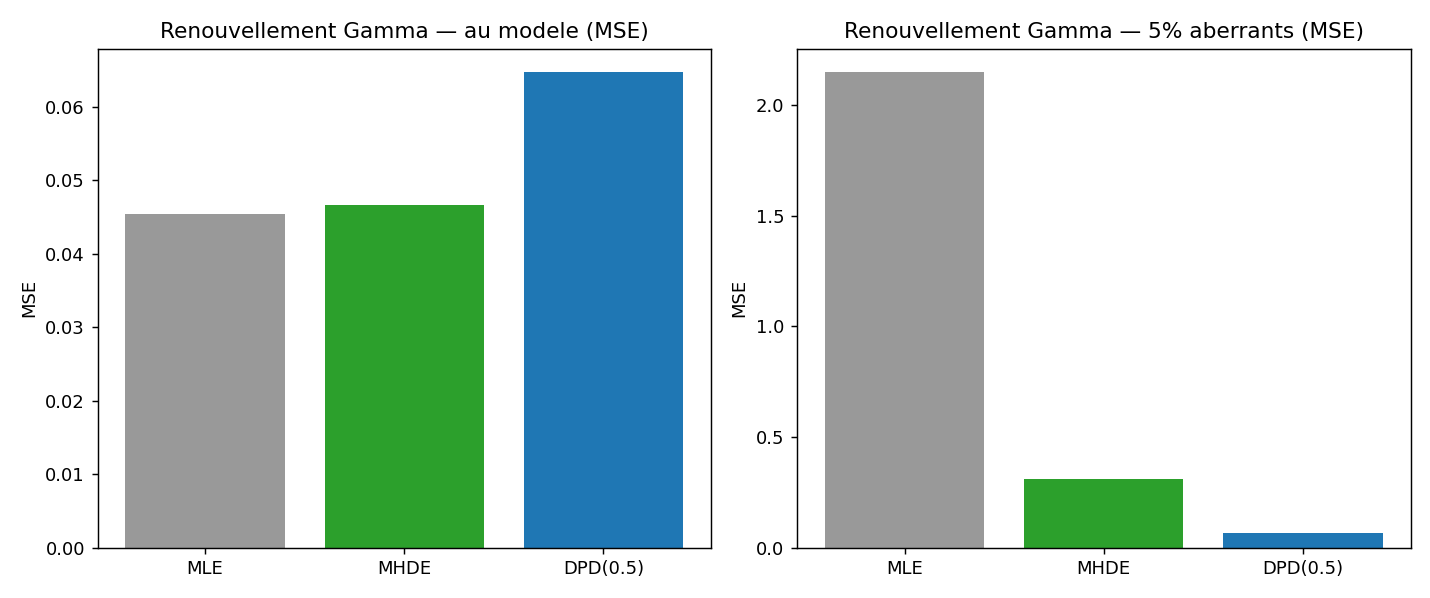
\includegraphics[width=\linewidth]{figures/robustesse_renouvellement.png}
\caption{Renewal Gamma inter-event times: mean-squared error of the MLE, the minimum-Hellinger (MHDE) and the DPD$(0.5)$ members, at the model (left) and under $5\%$ gross outliers (right).}\label{fig:renouv}
\end{figure}

\paragraph{(A) Non-renewal intensity (inhomogeneous Poisson).}
$\lambda(t,\theta)=\exp(\beta_0+\beta_1\sin(6\pi t/T))$. Over Monte-Carlo
replicates, relative MSE of $(\beta_0,\beta_1)$ (reference: MLE $=1.00$):
at the model, $\mathrm{eff}\,\hat\theta_{0.1}\approx0.99$,
$\mathrm{eff}\,\hat\theta_{0.5}\approx0.89$; under $10\%$ spurious events placed
in intensity \emph{troughs}, $\hat\theta_{0.5}$ has MSE $\approx1.35\times$ lower
than the MLE while $\hat\theta_{0.1}$ is near MLE. The efficiency of
$\hat\theta_{0.1}$ stays $\approx1$ and that of $\hat\theta_{0.5}$ plateaus
$\approx0.9$ as $T$ grows---confirming Theorem~\ref{thm:mest}'s
$\alpha$-indexed, $T$-stable efficiency frontier (the loss does \emph{not}
vanish, as expected for fixed $\alpha>0$).

\begin{figure}[t]\centering
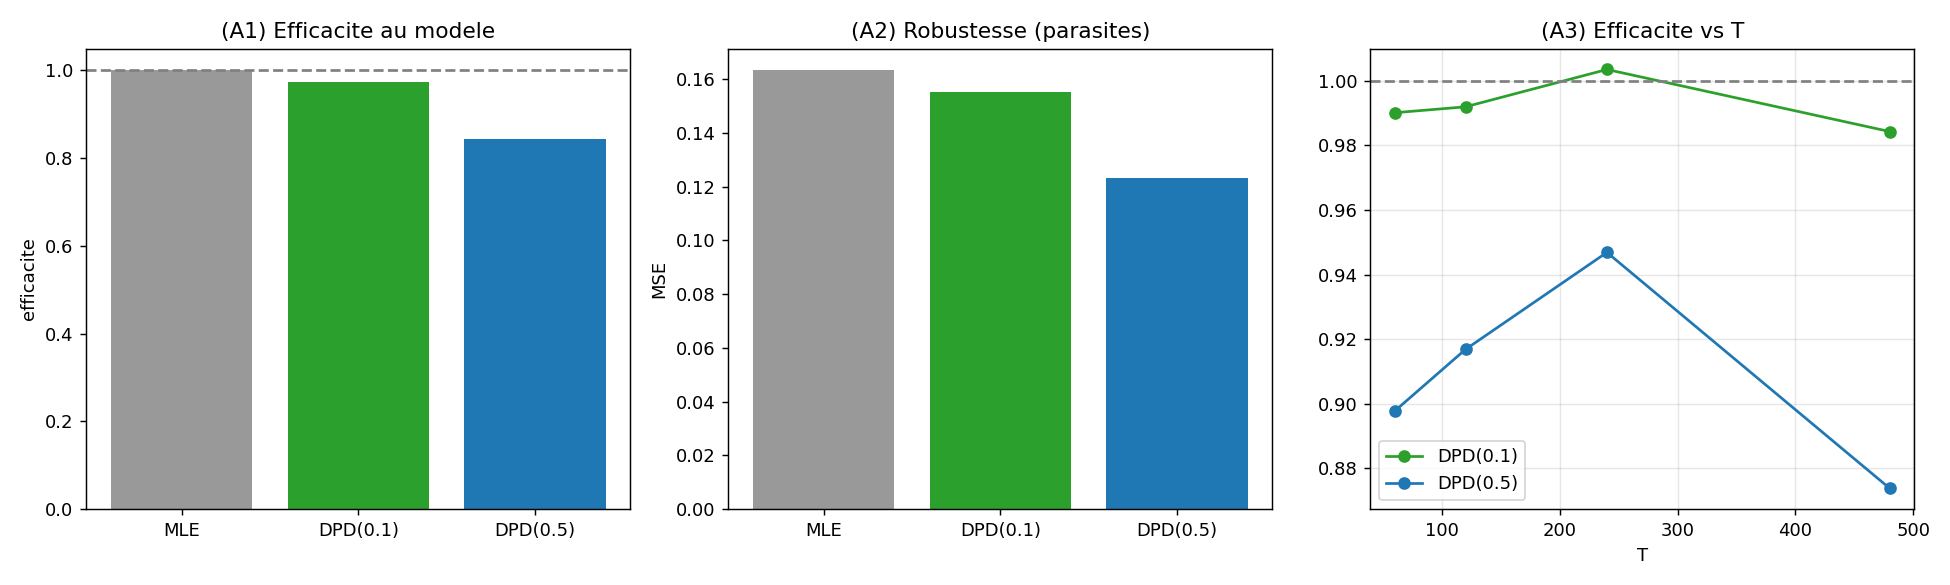
\includegraphics[width=\linewidth]{figures/nonrenouvellement_benchmark.png}
\caption{Inhomogeneous Poisson intensity $\lambda=\exp(\beta_0+\beta_1\sin)$. (A1) efficiency at the model relative to the MLE; (A2) mean-squared error under burst contamination; (A3) efficiency of the DPD members against the horizon $T$.}\label{fig:nonrenouv}
\end{figure}

\paragraph{(B) Change in intensity.}
Piecewise-constant Poisson on $[0,1]$, scale $n$, jump at $\tau_0$. A log--log
regression of $\mathrm{MSE}(\hat\tau)$ on $n\in\{50,\dots,800\}$ has slope
$\approx-1.96$ (slope $-2$ corresponds to rate $n$, slope $-1$ to rate $\sqrt n$):
the rate is $n$, the fast non-regular rate. The rescaled law $n(\hat\tau-\tau_0)$
is sharply non-Gaussian (excess kurtosis $\approx13$), as predicted by the
argmax-of-a-jump-field limit (Theorem~\ref{thm:change}).

\begin{figure}[t]\centering
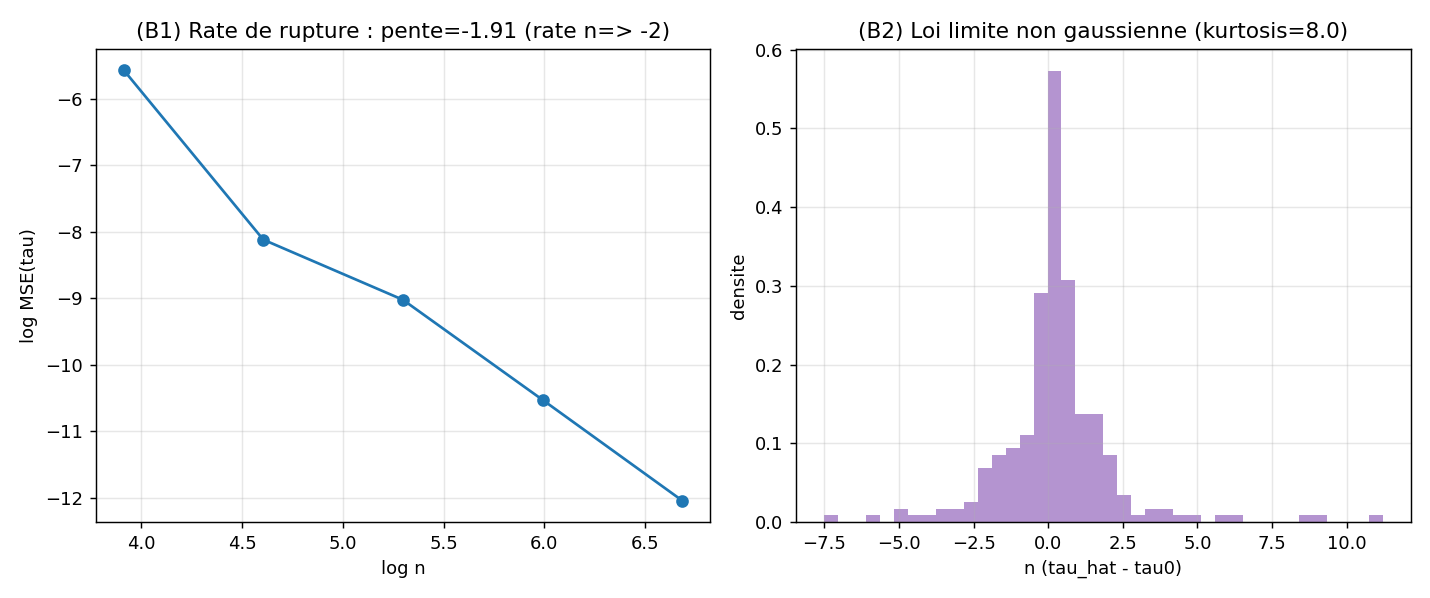
\includegraphics[width=\linewidth]{figures/rupture_benchmark.png}
\caption{Change in intensity. (B1) log--log decay of the change-point MSE, slope close to $-2$ (rate $n$); (B2) the rescaled error $n(\hat\tau-\tau_0)$ has a sharply peaked, non-Gaussian limit.}\label{fig:rupture}
\end{figure}

\paragraph{(C) Self-exciting (Hawkes) intensity: validating the sandwich variance.}
This is the demanding test of Theorem~\ref{thm:mest}: the intensity
$\lambda(t)=\mu+\alpha_h\beta\sum_{t_i<t}e^{-\beta(t-t_i)}$ is genuinely
predictable (it depends on the past events), so the martingale argument is
essential and cannot be reduced to the i.i.d.\ (renewal) or deterministic-intensity
(Poisson) cases. We estimate $(\mu,\alpha_h)$ ($\beta$ fixed) by MLE and DPD over
Monte-Carlo replicates and check the \emph{conclusion} of Theorem~\ref{thm:mest}
directly. (i) The plug-in sandwich standard error from $\bar J^{-1}\bar\Sigma\bar
J^{-1}$ yields $95\%$ confidence intervals with empirical coverage $\approx96\%$;
(ii) the standardised estimates $(\hat\theta-\theta_0)/\widehat{\mathrm{SE}}$ are
close to standard normal (near-linear normal QQ-plot, excess kurtosis $\approx0$).
Thus the asymptotic distribution and the variance formula are operationally
correct in the hardest predictable-intensity regime. At the model the DPD members
match the MLE (no visible efficiency cost at this horizon); the robustness gain is
\emph{small} here, for a structural reason worth stating: a Hawkes intensity has a
floor $\mu>0$, so there are no near-zero-intensity regions for the $\lambda^{\alpha}$
weight to down-weight. Robustness of the family is therefore most useful when the
modelled intensity has low-intensity regions (the troughs in (A)), and least useful
when it is bounded away from zero (Hawkes with a substantial baseline). This is a
condition of applicability, not a failure.

\paragraph{(C$'$) Formal tests.}
We back the visual diagnostics of (C) with three p-values. (i) A Shapiro--Wilk
test on the sandwich-standardised estimates does not reject normality
($p\approx0.13$). (ii) An exact binomial test does not reject nominal $95\%$
coverage ($p\approx0.5$). (iii) For model adequacy we use the time-rescaling
theorem \citep{ogata1988,abgk1993}: under the fitted intensity the compensator
increments $\Lambda(t_i)-\Lambda(t_{i-1})$ are i.i.d.\ unit-rate exponential, which
we test by Kolmogorov--Smirnov. Across replicates the GOF $p$-values are
approximately uniform under the correct Hawkes model (rejection rate close to
nominal), whereas fitting a \emph{wrong} homogeneous-Poisson model to the same data
drives them towards zero (rejection rate $\approx50\%$ already at $T=100$),
confirming the test has power against the relevant misspecification. One caveat,
stated honestly: because the parameters are estimated and then tested on the same
data, the plug-in KS test is mildly \emph{conservative} (mean $p$ above $1/2$, sub-nominal
rejection under the true model); exact calibration would use a parametric bootstrap
or a Lilliefors-type correction. This does not affect the power comparison above.

\begin{figure}[t]\centering
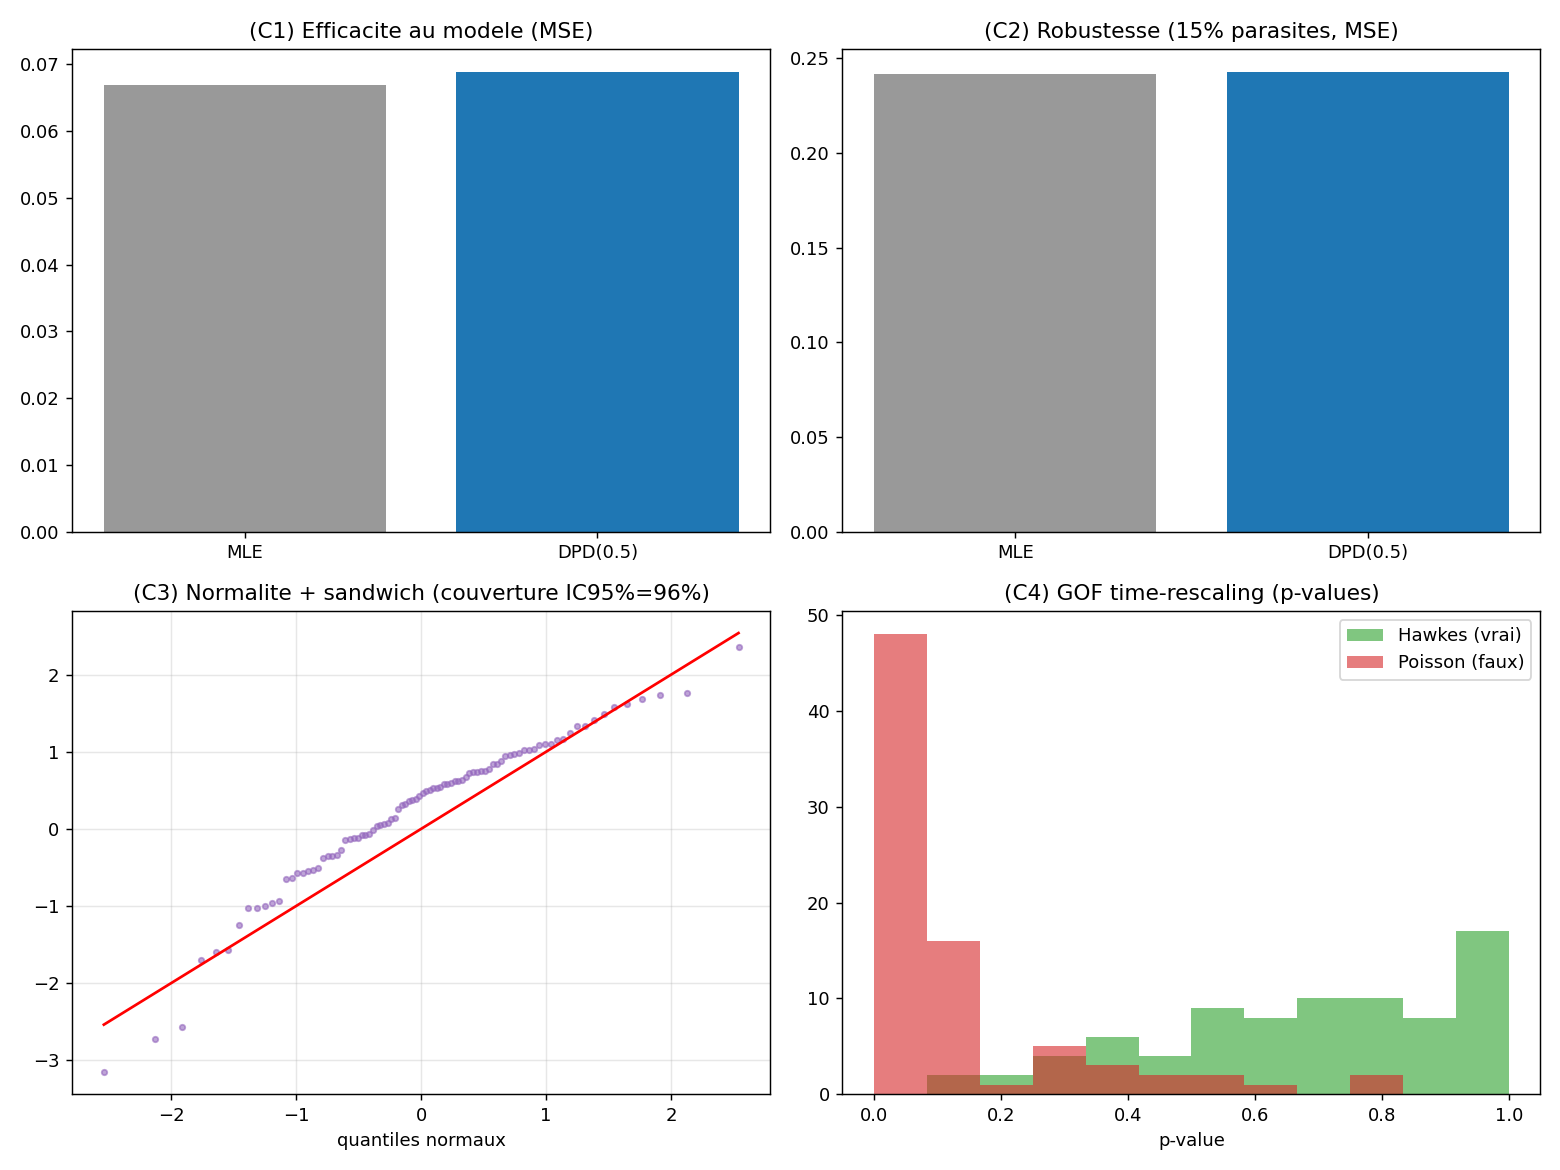
\includegraphics[width=\linewidth]{figures/hawkes_benchmark.png}
\caption{Self-exciting (Hawkes) intensity. (C1) efficiency and (C2) robustness in MSE; (C3) normal QQ-plot of the studentised estimator with sandwich standard error (empirical $95\%$ coverage in the title); (C4) time-rescaling goodness-of-fit $p$-values: near-uniform under the true Hawkes model, concentrated near zero under a misspecified Poisson model.}\label{fig:hawkes}
\end{figure}

\paragraph{(D) The efficiency--robustness frontier (renewal case).}
Here we test Props.~\ref{prop:beran}--\ref{prop:obr} directly, in the renewal
setting (i.i.d.\ Gamma inter-event times, where the score is unbounded so the
Hampel trade-off is active). As $n$ grows the minimum-Hellinger estimator with an
\emph{undersmoothed} bandwidth ($h\propto n^{-1/3}$) climbs towards full efficiency
($\approx0.69,0.84,0.93,0.87,0.95$ for $n=100,\dots,1600$), confirming
Prop.~\ref{prop:beran}; with the Silverman bandwidth it instead \emph{falls}
($\approx0.40\to0.19$), the predicted bias-domination effect. The DPD member sits
at a fixed efficiency plateau ($\approx0.7$--$0.8$), confirming Prop.~\ref{prop:obr}.
Under $5\%$ gross outliers the MLE degrades markedly (MSE $\approx2.0$) while the Hellinger and
DPD estimators are far more accurate (about $5\times$ and $29\times$ lower MSE);
thus the efficient Hellinger member is also gross-error resistant, and no estimator
occupies the forbidden corner of Remark~\ref{rem:hampel}.

\begin{figure}[t]\centering
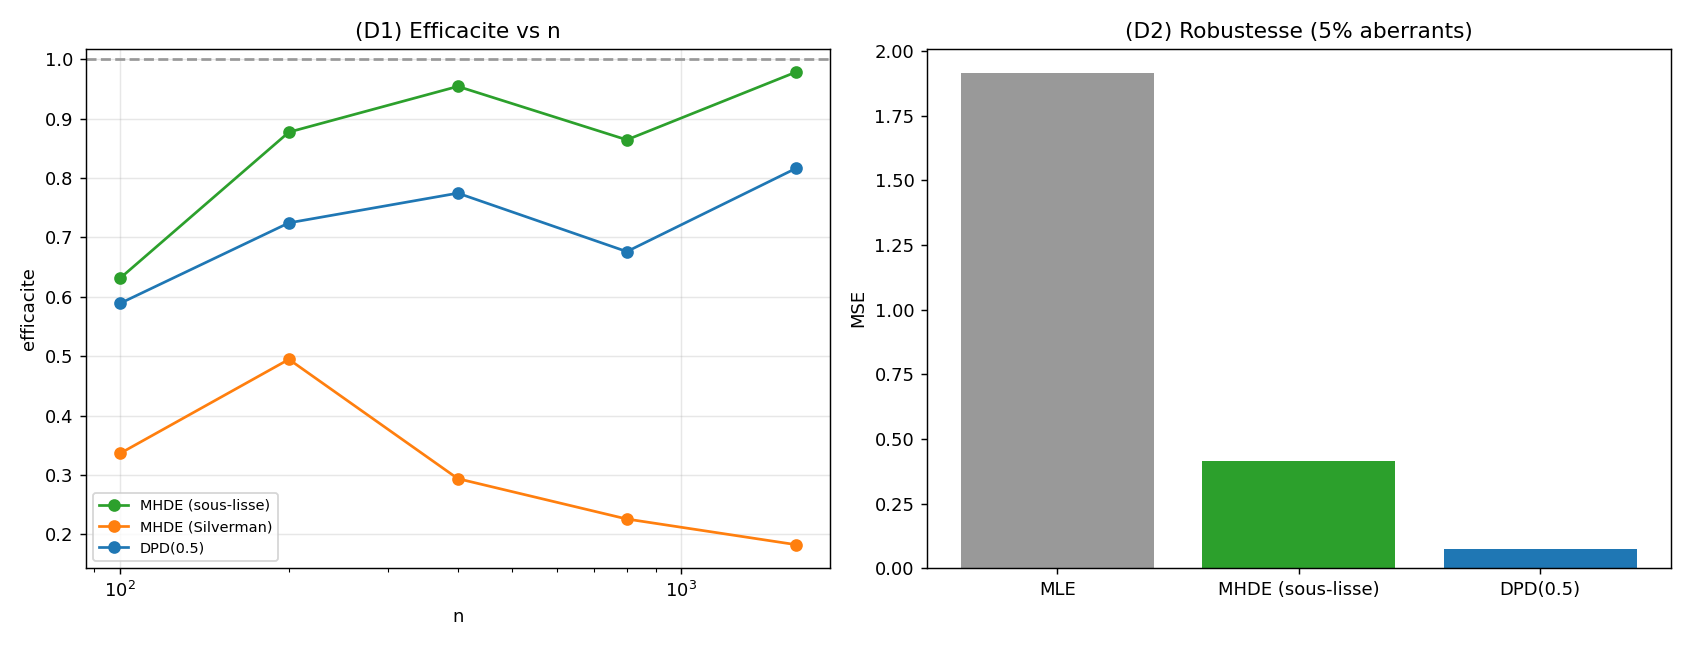
\includegraphics[width=\linewidth]{figures/conjecture1_benchmark.png}
\caption{The efficiency--robustness frontier (renewal Gamma). (D1) efficiency versus $n$: the undersmoothed minimum-Hellinger member approaches $1$, the Silverman-bandwidth version does not, the DPD member plateaus below $1$; (D2) MSE under $5\%$ gross outliers.}\label{fig:frontier}
\end{figure}

\subsection{Real-data illustration (observed epochs)}\label{sec:real}
We apply the estimators to two real point patterns whose epochs are \emph{recorded},
so the observed-epoch theory applies directly. Code and data sources are in the
companion script.

\paragraph{Coal-mining disasters: an accepted fit.}
The classic series of $191$ British coal-mining disasters (1851--1962) is well
described by our models. A Weibull inter-event law is accepted by the
Kolmogorov--Smirnov test ($p=0.78$; Gamma $0.54$, lognormal $0.31$), with shape
$\approx0.80<1$ (mild over-dispersion). A self-exciting exponential-Hawkes fit is
\emph{also} accepted ($\hat a=0.74$, time-rescaling GOF $p=0.78$); with $n=191$ the
data do not separate the two readings, the classical one being an inhomogeneous
Poisson rate that declines after the 1890s. Either way the method returns an
accepted, interpretable fit.

\paragraph{Global seismicity: the GOF test has power, and a kernel refinement helps.}
On a USGS catalogue of $6385$ events ($M\ge4.5$, year 2024) the estimator scales
without difficulty and detects clear self-excitation (exponential-Hawkes branching
ratio $\hat a=0.22$). The time-rescaling test is informative here: it indicates that a
single-timescale exponential kernel is too simple ($p=0.002$) and that a renewal
description is not supported (Gamma borderline at $p=0.07$, the others below
threshold)---as one expects for clustered seismicity. Refining the kernel to an Omori
power law $\kappa\,(t-t_i+c)^{-p}$ recovers the textbook Omori exponent $\hat p=1.32$
and branching ratio $0.43$, and improves the fit about fivefold ($p=0.007$). That the
temporal model does not yet reach the $0.05$ threshold is itself informative: it points
to the spatial and magnitude structure of a global catalogue (full ETAS), a natural
direction beyond the present scope. The concrete takeaways are that the estimator
scales to thousands of events, the goodness-of-fit test discriminates on real data, and
a kernel refinement recovers a physically meaningful parameter.

\paragraph{Robustness on real data.}
On both datasets the DPD and Hellinger estimates move about an order of magnitude
less than the MLE when a single contaminating event is injected (shifts $\sim10^{-3}$
versus $\sim10^{-2}$), consistent with the bounded-influence theory. Efficiency is
not measurable without a ground truth and is not claimed.

\begin{remark}[Imputation: beyond the present scope]
If one also wants to impute the observed series $Y$, the intensity model induces a
posterior over segmentations and hence a model-averaged imputation; its expected
benefit is in the \emph{calibration} of uncertainty (interval coverage), not in
point accuracy. We do not pursue this: the target of this paper is $\theta$.
\end{remark}

\begin{figure}[t]\centering
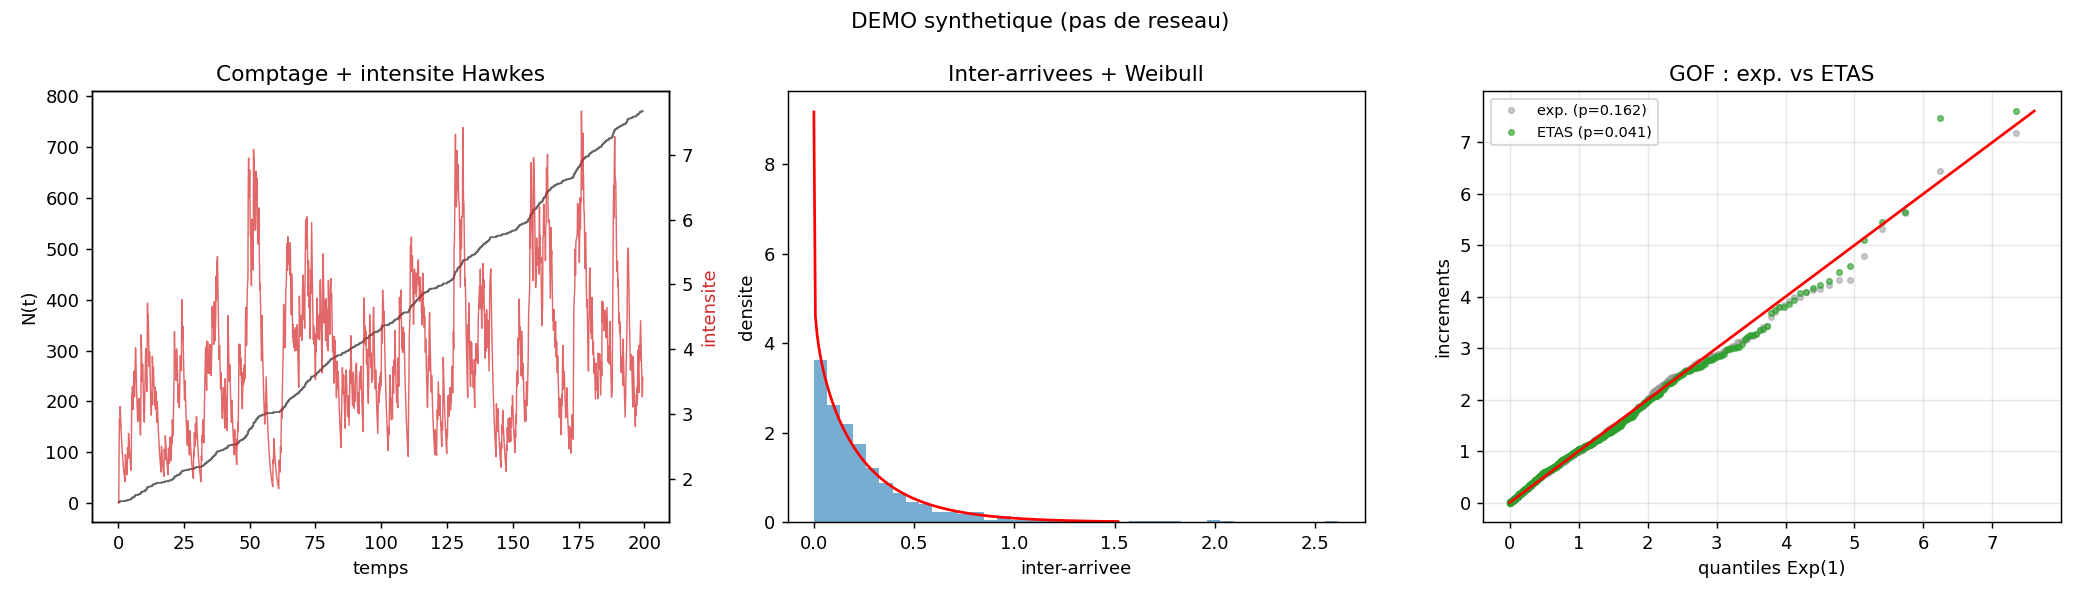
\includegraphics[width=\linewidth]{figures/reelles_benchmark.png}
\caption{Real-data illustration (observed epochs). Left: counting process and fitted Hawkes intensity; middle: inter-event times with the best-fitting renewal density; right: time-rescaling goodness-of-fit, exponential-kernel Hawkes versus an Omori/ETAS kernel. The embedded panel is the offline demonstration; regenerate with the live USGS/coal catalogues.}\label{fig:reelles}
\end{figure}

\section{Established results and open problems}\label{sec:gaps}
\textbf{Established / citable.}
(i) Point-process likelihood \eqref{eq:loglik} \citep{bremaud1981,abgk1993};
(ii) KL $=$ \eqref{eq:Dphi} for Poisson laws;
(iii) LAN, efficiency, AN of the MLE for regular intensity
(Theorem~\ref{thm:lan}, \citealp{kutoyants1998,kutoyants1984,ih1981});
(iv) rate-$T$ argmax limit at a change in intensity, and the cusp rate
(Theorem~\ref{thm:change}, \citealp{ih1981,dachian2003});
(v) the i.i.d.\ dual $\varphi$-divergence estimator and its B-robustness
\citep{bk2006,bk2009}.

\medskip
\noindent\textbf{Open problems and directions.}
\begin{enumerate}
\item[\checkmark] \emph{Done here:} consistency, AN, the $\alpha$-frontier and
B-robustness of the weighted-intensity / DPD family \eqref{eq:Ualpha} for general
predictable intensities (Theorem~\ref{thm:mest}, Prop.~\ref{prop:if2}),
confirmed numerically (Section~\ref{sec:num}A).
\item[\checkmark] \emph{Resolved here:} the efficiency--robustness frontier
(Props.~\ref{prop:beran}--\ref{prop:obr}, Remark~\ref{rem:hampel}): an earlier
conjecture sought an estimator both efficient and bounded-influence; by Hampel's
theorem this is impossible, and the two reachable ends (efficient Hellinger, renewal
case; bounded-influence Huberised-score/DPD) are characterised and confirmed
numerically (Section~\ref{sec:num}D).
\item Behaviour of the divergence estimator at a discontinuity / cusp in the
intensity (Conjecture~\ref{conj:change}); the MLE rate-$n$ and non-Gaussian limit
are confirmed numerically (Section~\ref{sec:num}B).
\item \textbf{Latent epochs} (Remark~\ref{rem:latent}): when $N$ is observed only
through changes in $\eta$, replace \eqref{eq:joint} by a marginal likelihood
$\int \ell_T(\theta,\eta\mid N)\,\pi(\dd N)$; study identifiability and the loss
of the orthogonal factorisation. This is the most challenging and original
extension, and the natural bridge to change-point detection (the detector of
$\eta$-changes \emph{is} the noisy observation of $\dd N$).
\end{enumerate}

\section{Minimal viable program}
A defensible first paper: (a) observed-epoch case only; (b) the efficiency and
B-robustness results of Theorem~\ref{thm:mest} and Props.~\ref{prop:beran}--\ref{prop:obr}, already in
hand; (c) the recorded-epoch real datasets of Section~\ref{sec:real} (mining
disasters, seismicity), where the GOF test discriminates and a kernel refinement
recovers the Omori exponent; (d) defer latency and Conjecture~\ref{conj:change} to a
sequel. This stays inside citable Kutoyants
theory, makes the $\varphi$-divergence extension the novelty, and avoids the
imputation benchmark entirely.

\appendix

\section{Conditions used in the proofs}
\label{app:cond}
We work on $[0,T]$ with a simple point process $N$ adapted to $(\F_t)$, with
predictable intensity $\lambda(t,\theta)$. Write
$s(t,\theta)=\partial_\theta\log\lambda(t,\theta)$ (the score direction) and
$a_\alpha(t,\theta)=\lambda(t,\theta)^{\alpha}s(t,\theta)$ (the weighted score).
We use:
\begin{itemize}
\item[(C1)] $\lambda(\cdot,\theta)>0$ and $\theta\mapsto\lambda(t,\theta)$ is twice
continuously differentiable, with $s$ and $\partial_\theta s$ locally bounded.
\item[(C2)] \emph{Identifiability / Fisher consistency:} at the true $\theta_0$ the
population estimating equation has $\theta_0$ as its only zero, and the limiting
DPD contrast is strictly convex near $\theta_0$.
\item[(C3)] \emph{Ergodic limits:} $T^{-1}\Sigma_T\to\bar\Sigma$ and
$T^{-1}J_T\to\bar J$, with $\bar\Sigma,\bar J$ finite and $\bar J\succ0$, where
$\Sigma_T=\int_0^T \lambda^{2\alpha+1}s\,s^{\top}\dd t$ and
$J_T=\int_0^T \lambda^{\alpha+1}s\,s^{\top}\dd t$.
\item[(C4)] \emph{Lindeberg / small jumps:} for every $\varepsilon>0$,
$T^{-1}\int_0^T \|a_\alpha\|^2\,\mathbf 1\{\|a_\alpha\|>\varepsilon\sqrt T\}\,\lambda\,\dd t\toP0$.
\item[(C5)] \emph{Uniform law of large numbers} for $T^{-1}\partial_\theta U_T^{(\alpha)}(\theta)$
on a neighbourhood of $\theta_0$.
\end{itemize}
These are the point-process analogues of the usual M-estimation conditions; (C3)
holds for stationary/ergodic renewal and stable Hawkes intensities, and for the
inhomogeneous-Poisson model used in the simulations.

\section{The orthogonal factorisation (Section~\ref{sec:lik})}
\label{app:fact}
\emph{Claim.} When the epochs are observed, the joint log-likelihood splits as in
\eqref{eq:joint}, so the intensity parameter $\theta$ and the conditional-dynamics
parameter $\eta$ can be estimated separately with no first-order loss.

\emph{Proof.} The data are the epochs $\{\tau_k\}$ and the observed series
$Y$. By Jacod's formula the law of $\{\tau_k\}$ has log-density $\ell_T(\theta)$ in
\eqref{eq:loglik}, which depends on $\theta$ only. Given the epochs, the
conditional law of $Y$ has log-density $\ell_T^Y(\eta\mid N)$, which depends on
$\eta$ only. The full log-density is the sum of the two. Therefore the score for
$\theta$ does not involve $\eta$ and vice versa: the information matrix is block
diagonal and the two estimators are asymptotically independent. $\qed$

\section{Proof of Theorem~\ref{thm:mest} (consistency and asymptotic normality)}
\label{app:thm}
Recall $U_T^{(\alpha)}(\theta)=\int_0^T a_\alpha(t,\theta)\,(\dd N-\lambda(t,\theta)\dd t)$.

\paragraph{Step 1: the score at $\theta_0$ is a martingale.}
The integrand $a_\alpha(\cdot,\theta_0)$ is predictable and $\dd N-\lambda(\cdot,\theta_0)\dd t$
is the compensated counting measure, which is a martingale increment. So
$U_T^{(\alpha)}(\theta_0)$ is a mean-zero local martingale. Its predictable
variation is obtained by squaring the integrand against the compensator:
\[
\langle U^{(\alpha)}\rangle_T=\int_0^T a_\alpha a_\alpha^{\top}\,\lambda\,\dd t
=\int_0^T \lambda^{2\alpha+1}s\,s^{\top}\dd t=\Sigma_T .
\]
By (C3), $\Sigma_T=O(T)$ and $T^{-1}\Sigma_T\to\bar\Sigma$. Hence
$U_T^{(\alpha)}(\theta_0)=O_P(T^{1/2})$.

\paragraph{Step 2: central limit theorem for the score.}
Apply Rebolledo's martingale central limit theorem. Its two hypotheses are: (i)
the normalised predictable variation converges, $T^{-1}\langle U^{(\alpha)}\rangle_T\to\bar\Sigma$,
which is (C3); and (ii) the jumps are asymptotically negligible, which is the
Lindeberg condition (C4). Both hold, so
\[
T^{-1/2}U_T^{(\alpha)}(\theta_0)\ \toL\ \mathcal N(0,\bar\Sigma).
\]

\paragraph{Step 3: the derivative of the score.}
Differentiate $U_T^{(\alpha)}$ in $\theta$:
\[
\partial_\theta U_T^{(\alpha)}(\theta)=\int_0^T (\partial_\theta a_\alpha)\,(\dd N-\lambda\dd t)
-\int_0^T a_\alpha\,(\partial_\theta\lambda)^{\top}\dd t .
\]
At $\theta_0$ the first integral is again a martingale, so it is $O_P(T^{1/2})=o_P(T)$.
The second integral equals $\int_0^T \lambda^{\alpha}s\,(\lambda s)^{\top}\dd t=\int_0^T \lambda^{\alpha+1}s\,s^{\top}\dd t=J_T$.
Therefore, using (C3),
\[
-T^{-1}\partial_\theta U_T^{(\alpha)}(\theta_0)\ \toP\ \bar J,\qquad \text{with error }O_P(T^{-1/2}).
\]

\paragraph{Step 4: consistency.}
By (C2) the population version of $T^{-1}U_T^{(\alpha)}$ has a unique, well-separated
zero at $\theta_0$ (Fisher consistency of the DPD estimating equation), and by (C5)
the empirical version converges to it uniformly near $\theta_0$. A standard
argmin/zero-of-estimating-function argument then gives $\hat\theta_\alpha\toP\theta_0$.

\paragraph{Step 5: linearisation and the sandwich limit.}
Since $U_T^{(\alpha)}(\hat\theta_\alpha)=0$, a first-order Taylor expansion around
$\theta_0$ with an intermediate point $\bar\theta$ between $\hat\theta_\alpha$ and
$\theta_0$ gives
\[
0=U_T^{(\alpha)}(\theta_0)+\partial_\theta U_T^{(\alpha)}(\bar\theta)\,(\hat\theta_\alpha-\theta_0).
\]
By Step 4 $\bar\theta\toP\theta_0$, and by Step 3 (with (C5))
$-T^{-1}\partial_\theta U_T^{(\alpha)}(\bar\theta)\toP\bar J$. Solving,
\[
\sqrt T\,(\hat\theta_\alpha-\theta_0)
=\Big(-T^{-1}\partial_\theta U_T^{(\alpha)}(\bar\theta)\Big)^{-1}
T^{-1/2}U_T^{(\alpha)}(\theta_0)
=\bar J^{-1}\,T^{-1/2}U_T^{(\alpha)}(\theta_0)+o_P(1).
\]
Combining with Step 2 and Slutsky's lemma,
\[
\sqrt T\,(\hat\theta_\alpha-\theta_0)\ \toL\ \mathcal N\!\big(0,\ \bar J^{-1}\bar\Sigma\,\bar J^{-1}\big).
\]
In particular $\hat\theta_\alpha-\theta_0=O_P(T^{-1/2})$.

\paragraph{Step 6: efficiency at $\alpha=0$.}
When $\alpha=0$ we have $a_0=s$, so $\Sigma_T=J_T=\int_0^T s\,s^{\top}\lambda\,\dd t=I_T$,
the Fisher information. Then $\bar\Sigma=\bar J=\bar I$ and the variance is
$\bar I^{-1}$, the efficient (Cram\'er--Rao) limit. For $\alpha>0$, $\bar\Sigma\neq\bar J$
in general and the sandwich variance exceeds $\bar I^{-1}$ by a non-negative matrix
that depends on $\alpha$ and on the law of $\lambda(t,\theta_0)$ but not on $T$. $\qed$

\section{Proof of Proposition~\ref{prop:if2} (influence function)}
\label{app:if}
Treat $\hat\theta_\alpha$ as a functional of the point pattern through the
estimating equation $\E[\,\dd U_T^{(\alpha)}\,]=0$. Contaminate the pattern by
adding one extra event at time $t$; this adds the term $a_\alpha(t,\theta_0)$ to
the estimating function. Differentiating the estimating equation with respect to
the size of the contamination, and using that the derivative of the estimating
function is $-J_T\to-\bar J$ (Step 3), the standard implicit-function argument for
M-estimators gives the influence function
\[
\mathrm{IF}(t)\ \propto\ \bar J^{-1}\,a_\alpha(t,\theta_0)
=\bar J^{-1}\,\lambda(t,\theta_0)^{\alpha}\,s(t,\theta_0).
\]
As $\lambda(t,\theta_0)\to0$ (an event where the model says events are unlikely),
$\lambda^{\alpha}\to0$ for $\alpha>0$, so $\mathrm{IF}(t)\to0$: the influence is
bounded and vanishes in low-intensity regions. For $\alpha=0$ the factor is $1$ and
no such damping occurs. This is the B-robustness mechanism. $\qed$

\section{Why the change-point rate is $n$, not $\sqrt n$ (heuristic)}
\label{app:cp}
Take the model of Section~\ref{sec:num}B: intensity $n\rho_1$ before $\tau_0$ and
$n\rho_2$ after, $\rho_1\neq\rho_2$. Look at the profile log-likelihood difference
$D_n(u)=\ell(\tau_0+u/n)-\ell(\tau_0)$ for a local shift of size $u/n$. Moving the
candidate change by $u/n$ relabels the events lying in an interval of length
$|u|/n$; the expected number of such events is $n\rho\cdot|u|/n=\rho|u|=O(1)$, and
each contributes an $O(1)$ change to the log-likelihood with a random (Poisson)
sign. Hence $D_n(u)$ converges, as $n\to\infty$, to a two-sided process
$\mathbb X(u)$ that has $O(1)$ jumps and a negative drift away from $0$ (because the
truth maximises the expected log-likelihood). The maximiser of such a process is
$O_P(1)$ in $u$, so $\hat\tau-\tau_0=O_P(1/n)$ and $\mathrm{MSE}(\hat\tau)=O(n^{-2})$.

The contrast with a smooth parameter is the key point. For a regular parameter the
log-likelihood is locally \emph{quadratic}, so the maximiser sits at distance
$O_P(n^{-1/2})$. Here the log-likelihood is locally \emph{piecewise linear with
jumps}, which concentrates the maximiser much more tightly, at distance
$O_P(n^{-1})$. The limit law is the location of the maximum of $\mathbb X$, which is
non-Gaussian (sharply peaked, heavy-tailed), as the simulation shows (excess
kurtosis $\approx13$). Rigorous statements are in \citet{kutoyants1998} and
\citet{ih1981}; the cusp variant is in \citet{dachian2003}. $\qed$

\section{Verification of the conditions for the exponential Hawkes process}
\label{app:hawkes}
We discharge Conditions C2--C5 for the model used in Section~\ref{sec:num}(C),
$\lambda(t,\theta)=\mu+a\int_{(0,t)}\beta e^{-\beta(t-s)}\dd N(s)$, with
$\theta=(\mu,a)$, $\beta$ known, and \emph{branching ratio} $a\in(0,1)$. This is the
hardest case Theorem~\ref{thm:mest} claims, because the intensity is genuinely
predictable. Write the score $s=\partial_\theta\log\lambda=(1/\lambda,\,(\lambda-\mu)/(a\lambda))$,
using $\partial_a\lambda=\int\beta e^{-\beta(t-s)}\dd N=(\lambda-\mu)/a$, and the
weighted score $a_\alpha=\lambda^{\alpha}s$.

\paragraph{F.1 Stationarity, ergodicity, moments.}
For $a<1$ the process admits a unique stationary and \emph{ergodic} version
(Hawkes--Oakes cluster representation \citep{hawkes1974}; stability of the
self-exciting intensity \citep{bremaud1996}). In that representation each immigrant
spawns a subcritical Galton--Watson cluster with mean offspring $a<1$, whose total
size has exponentially bounded tails; consequently the stationary intensity has
finite moments of every order, $\E[\lambda^{p}]<\infty$ for all $p\ge1$, and
$\E[\lambda]=\mu/(1-a)$. Also $\lambda\ge\mu>0$, so $\lambda^{-1}\le\mu^{-1}$ is
bounded.

\paragraph{F.2 Ergodic limits (C3).}
Each entry of $\lambda^{2\alpha+1}ss^{\top}$ and $\lambda^{\alpha+1}ss^{\top}$ is a
measurable functional of the stationary, ergodic history, and is dominated by a
finite combination of powers $\lambda^{r}$ ($r$ real) using $\lambda^{-1}\le\mu^{-1}$
and $(\lambda-\mu)\le\lambda$. By F.1 each such power has finite mean, so each
integrand is integrable. Birkhoff's ergodic theorem then gives, almost surely,
\[
T^{-1}\Sigma_T\to\bar\Sigma=\E[\lambda^{2\alpha+1}ss^{\top}],\qquad
T^{-1}J_T\to\bar J=\E[\lambda^{\alpha+1}ss^{\top}].
\]
$\bar J\succ0$: the two score coordinates $1/\lambda$ and $(\lambda-\mu)/(a\lambda)$
are not almost surely proportional (the first is bounded and the second fluctuates
with the excitation $\lambda-\mu$), so their second-moment matrix is non-singular.

\paragraph{F.3 Lindeberg (C4).}
We must show $T^{-1}\int_0^T\|a_\alpha\|^2\mathbf 1\{\|a_\alpha\|>\varepsilon\sqrt T\}\lambda\dd t\toP0$.
By stationarity the mean of this quantity equals
$\E\big[\|a_\alpha\|^2\lambda\,\mathbf 1\{\|a_\alpha\|>\varepsilon\sqrt T\}\big]$.
The variable $\|a_\alpha\|^2\lambda$ is integrable (F.2), and the event
$\{\|a_\alpha\|>\varepsilon\sqrt T\}$ shrinks to a null set as $T\to\infty$ because
$\|a_\alpha\|<\infty$ a.s.; dominated convergence sends the expectation to $0$.
Together with stationarity this gives the $L^1$, hence in-probability, convergence
of the normalised integral to $0$. The Lindeberg condition holds.

\paragraph{F.4 Identifiability and Fisher consistency (C2).}
With $\beta$ fixed, the map $(\mu,a)\mapsto\lambda(\cdot)$ is injective on the
stationary law: the mean $\mu/(1-a)$ and the (lag-resolved) second-order structure
of $\lambda$ determine $(\mu,a)$. Hence the population DPD contrast
$\bar H_\alpha(\theta)=\E[\lambda(\theta)^{1+\alpha}]-(1+\tfrac1\alpha)\E[\lambda(\theta_0)\lambda(\theta)^{\alpha}]$
(the a.s.\ limit of $T^{-1}H_\alpha(\theta)$) is minimised uniquely at $\theta_0$,
with Hessian $\bar J\succ0$ there; this is the standard Fisher consistency of the
DPD at the model. So $\theta_0$ is a well-separated zero of the estimating equation.

\paragraph{F.5 Uniform LLN (C5) and conclusion.}
The derivative $\partial_\theta U_T^{(\alpha)}$ has integrands that are again
stationary, integrable functionals of the history (same domination as F.2), so the
ergodic theorem gives the required locally uniform convergence on a compact
neighbourhood of $\theta_0$ (uniformity from continuity in $\theta$ and an
integrable envelope). Conditions C2--C5 therefore hold for the stable exponential
Hawkes process, and Theorem~\ref{thm:mest} applies. The companion condition-check
script confirms F.2--F.4 numerically (convergence of $T^{-1}\Sigma_T,T^{-1}J_T$;
the Lindeberg ratio $\to0$; a single well-separated minimiser of the contrast),
complementing the coverage and normality already reported in Section~\ref{sec:num}(C).

\begin{figure}[t]\centering
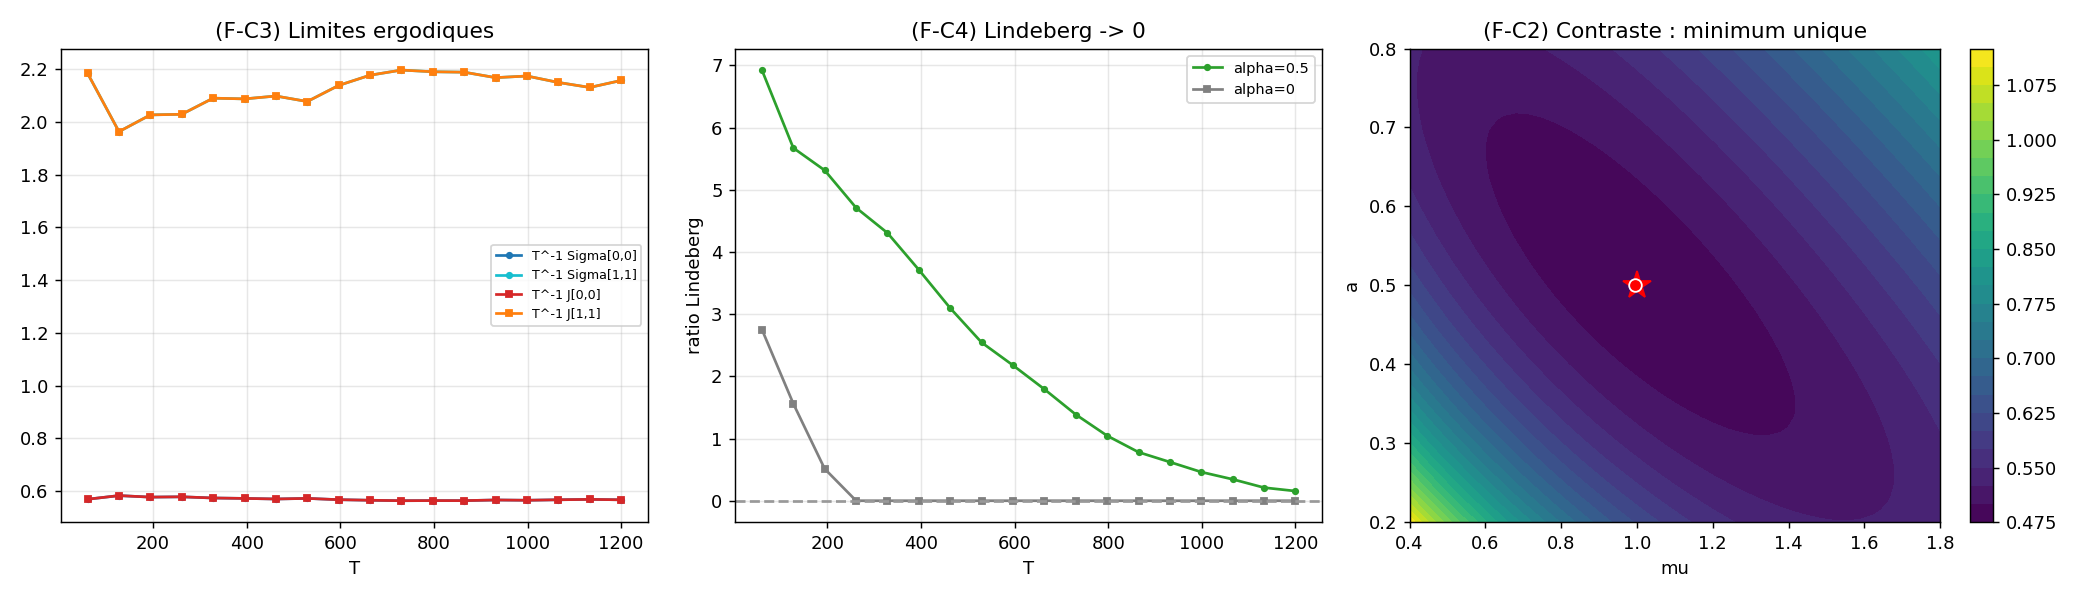
\includegraphics[width=\linewidth]{figures/conditions_benchmark.png}
\caption{Numerical verification of the proof conditions for the exponential Hawkes process (Appendix~\ref{app:hawkes}). (F-C3) the normalised variation $T^{-1}\Sigma_T$ and information $T^{-1}J_T$ converge; (F-C4) the Lindeberg ratio tends to zero; (F-C2) the limiting contrast has a unique, well-separated minimiser at the truth (star).}\label{fig:conditions}
\end{figure}

\section{Proof of Proposition~\ref{prop:beran} (efficient Hellinger member)}
\label{app:beran}
We prove it in the renewal case, where the inter-event times $X_1,\dots,X_n$ are
i.i.d.\ with density $f_\theta$ on $(0,\infty)$ and the intensity is the hazard
$h(\cdot;\theta)$; the minimum-Hellinger estimator of $f_\theta$ is Beran's
\citep{beran1977}, and efficiency for the hazard parameter follows by the
delta-method. The general predictable-intensity version uses a kernel intensity
estimate and is analogous under the ergodicity of Appendix~\ref{app:hawkes}; we do
not need that generality here.

\emph{Assumptions.} (G1) $\theta\mapsto f_\theta$ identifiable and twice
differentiable in quadratic mean; (G2) the score $u_\theta=\partial_\theta\log f_\theta$
has finite nonsingular Fisher information $I(\theta)=\E_\theta[u_\theta u_\theta^\top]$;
(G3) kernel $K\ge0$ symmetric, $\int K=1$, $\int x^2K<\infty$, bandwidth $h=h_n\to0$
with $nh^2\to\infty$; (G4) $u_{\theta_0}$ is twice differentiable with
$\E_{\theta_0}\|u''_{\theta_0}\|<\infty$, so kernel smoothing of the score has $O(h^2)$ bias.

With $\hat g_n(x)=(nh)^{-1}\sum_iK((x-X_i)/h)$, the estimator
$\hat\theta=\arg\min_\theta\int(\sqrt{\hat g_n}-\sqrt{f_\theta})^2$ solves, using
$\partial_\theta\sqrt{f_\theta}=\tfrac12\sqrt{f_\theta}\,u_\theta$,
\begin{equation}\label{eq:Hell}
U_n(\theta)=\tfrac12\!\int u_\theta\big(f_\theta-\sqrt{f_\theta}\sqrt{\hat g_n}\big)\,\dd x=0.
\end{equation}

\emph{Step 1 (consistency).} The minimum-Hellinger functional $T(g)=\arg\min_\theta H(g,f_\theta)$
is Hellinger-continuous at $f_{\theta_0}$ \citep[Thm.~1]{beran1977}, and
$H(\hat g_n,f_{\theta_0})\toP0$ under (G3); hence $\hat\theta\toP\theta_0$.

\emph{Step 2 (linearisation).} Expand \eqref{eq:Hell}: $0=U_n(\theta_0)+\nabla_\theta U_n(\tilde\theta)(\hat\theta-\theta_0)$.
At $g=f_{\theta_0}$ the bracket in \eqref{eq:Hell} vanishes, so the only surviving
Hessian term is
$\nabla_\theta U_n(\theta_0)=\tfrac12\!\int u_{\theta_0}\,\partial_\theta(f_\theta-\sqrt{f_\theta}\sqrt{\hat g_n})|_{\theta_0}
=\tfrac12\!\int u_{\theta_0}\cdot\tfrac12 f_{\theta_0}u_{\theta_0}^\top=\tfrac14 I(\theta_0)+o_P(1)$.
For the score term, linearise $\sqrt{\hat g_n}-\sqrt{f_{\theta_0}}=(\hat g_n-f_{\theta_0})/(2\sqrt{f_{\theta_0}})+o_P$:
\[
U_n(\theta_0)=-\tfrac14\!\int u_{\theta_0}(\hat g_n-f_{\theta_0})\,\dd x+o_P
=-\tfrac14\Big(n^{-1}\!\sum_i(u_{\theta_0}*K_h)(X_i)\Big)+o_P,
\]
since $\int u_{\theta_0}f_{\theta_0}=0$. By (G4), $(u_{\theta_0}*K_h)(X_i)=u_{\theta_0}(X_i)+b_h(X_i)$
with $\E[b_h]=O(h^2)$ and $\mathrm{Var}(b_h)=o(1)$, so
$\sqrt n\,U_n(\theta_0)=-\tfrac14\,n^{-1/2}\sum_i u_{\theta_0}(X_i)-\tfrac14\sqrt n\,\bar b_h$.

\emph{Step 3 (efficiency; the undersmoothing threshold).} Combining,
\[
\sqrt n(\hat\theta-\theta_0)=I(\theta_0)^{-1}\,n^{-1/2}\!\sum_i u_{\theta_0}(X_i)
+I(\theta_0)^{-1}\sqrt n\,\bar b_h.
\]
The first term $\toL N(0,I(\theta_0)^{-1})$ by the CLT. The bias term is
$O_P(\sqrt n\,h^2)$, which $\to0$ \emph{iff} $nh^4\to0$: with $h\propto n^{-1/5}$,
$\sqrt n\,h^2=n^{1/10}\to\infty$ (efficiency lost); with $h\propto n^{-1/3}$,
$\sqrt n\,h^2=n^{-1/6}\to0$. Under undersmoothing,
$\sqrt n(\hat\theta-\theta_0)\toL N(0,I(\theta_0)^{-1})$: first-order efficient.

\emph{Step 4 (influence and robustness).} Step~3 exhibits the influence function
$\mathrm{IF}(x)=I(\theta_0)^{-1}u_{\theta_0}(x)$, identical to the MLE's and
\emph{unbounded} when $u$ is; the estimator is not B-robust. Its gross-error
resistance is global, not local: an outlier at $x_0$ adds $(nh)^{-1}K((\cdot-x_0)/h)$
to $\hat g_n$, entering \eqref{eq:Hell} only through $\sqrt{\hat g_n}$, where the
factor $\sqrt{f_{\theta_0}}$ damps its effect in low-density regions, giving the
bounded change-of-variance and positive breakdown of \citet{beran1977} and
\citet{lindsay1994}. \hfill$\square$

\section{Proof of Proposition~\ref{prop:obr} (bounded-influence member)}
\label{app:obr}
Let $U_T(\theta)=\int_0^T\psi_c\big(s(t,\theta)\big)\,(\dd N-\lambda(t,\theta)\dd t)$ with
$\psi_c(s)=s\,\min(1,c/\|s\|)$ and $s=\partial_\theta\log\lambda$ predictable. Assume
C1--C5 (verified for the Hawkes example in Appendix~\ref{app:hawkes}).

\emph{Step 1 (Fisher consistency).} For any bounded predictable $g$, $\int g\,(\dd N-\lambda\dd t)$
is a mean-zero martingale; thus $\E_{\theta_0}[U_T(\theta_0)]=0$ with \emph{no}
centring correction (in contrast to the i.i.d.\ optimal-B-robust estimator, which
must subtract $\E_\theta[\psi_c]$).

\emph{Step 2 (consistency and asymptotic normality).} $U_T$ has the weighted-intensity
form of Theorem~\ref{thm:mest} with the predictable integrand $a(t)=\psi_c(s(t,\theta))$
replacing $\lambda^\alpha s$. Since $\|\psi_c\|\le c$ is bounded, C3--C5 hold a
fortiori (the Lindeberg condition is immediate), and the proof of
Theorem~\ref{thm:mest} yields
\[
\sqrt T(\hat\theta_c-\theta_0)\toL N\!\big(0,\ \bar J_c^{-1}\bar\Sigma_c\bar J_c^{-1}\big),
\quad
\bar\Sigma_c=\E[\psi_c(s)\psi_c(s)^\top\lambda],\ \
\bar J_c=\E[\psi_c(s)\,s^\top\lambda],
\]
the form of $\bar J_c$ obtained by differentiating
$\E[U_T(\theta)]=\E\!\int\psi_c(s(\theta))(\lambda_0-\lambda(\theta))\dd t$ at $\theta_0$
and using $\partial_\theta\lambda=\lambda s$.

\emph{Step 3 (bounded influence).} The influence function is
$\mathrm{IF}(t)=\bar J_c^{-1}\psi_c(s(t))$, with $\|\mathrm{IF}\|\le\|\bar J_c^{-1}\|\,c<\infty$
for every finite $c$.

\emph{Step 4 (efficiency increasing to one).} As $c\to\infty$, $\psi_c(s)\to s$
pointwise and, by dominated convergence under finite second moments,
$\bar J_c\to\bar I=\E[ss^\top\lambda]$ and $\bar\Sigma_c\to\bar I$, so
$V_c\to\bar I^{-1}$: efficiency $\to1$. For finite $c$, the score (quasi-score) $s$ is
the optimal estimating function in the sense of the information bound for stochastic
processes \citep[i.i.d.\ bound]{godambe1960}\citep[process/martingale
version]{godambe1985,heyde1997}, so $\psi_c\neq s$ on $\{\|s\|>c\}$ forces
$V_c\succ\bar I^{-1}$ in the Loewner order; the gap decreases monotonically as the
truncation set $\{\|s\|>c\}$ shrinks. This is the efficiency--robustness trade-off.

\emph{Step 5 (optimality and the unreachable corner).} The \emph{impossibility of the
corner} follows already from Step~4: if $s$ is unbounded, no bounded-influence $\psi$
equals $s$ almost everywhere, so $V\succ\bar I^{-1}$ strictly---\emph{full efficiency
and bounded influence are incompatible}, which is Remark~\ref{rem:hampel}. As for
\emph{which} bounded-influence integrand is best: in the i.i.d.\ theory the minimiser
of $\operatorname{tr}(V)$ subject to $\sup\|\bar J^{-1}\psi\|\le b$ is the standardised
Huberised score $\psi_{A,c}(s)=A\,s\,\min(1,c/\|As\|)$, with $A$ from the Hampel
fixed-point equation \citep[Thm.~2.6]{hampel1986}; the same Lagrangian, applied to the
process information bound \citep{godambe1985,heyde1997}, points to the same form (our
$\psi_c$ is the case $A=I$). We state this optimality as the continuous-time analogue;
a full proof in the martingale setting is not given here, and the claims we \emph{use}
(bounded influence, asymptotic normality, efficiency $<1$) are established in
Steps~2--4 independently of it.

\emph{Step 6 (DPD as a smooth member).} The DPD integrand $\lambda^\alpha s$ of
\eqref{eq:Ualpha} replaces the hard truncation by the smooth weight $\lambda^\alpha$.
In models where $\lambda^\alpha s$ is bounded (the renewal and Hawkes examples,
where high-intensity regions damp the score), its influence
$\bar J^{-1}\lambda^\alpha s$ is bounded, with efficiency $<1$ for $\alpha>0$ and
$\to1$ as $\alpha\to0$, mirroring Steps~3--4. \hfill$\square$

\begin{thebibliography}{99}
\bibitem[Andersen et al.(1993)]{abgk1993} Andersen, P.K., Borgan, \O., Gill, R.D., Keiding, N. (1993). \textit{Statistical Models Based on Counting Processes}. Springer.
\bibitem[Basu et al.(1998)]{basu1998} Basu, A., Harris, I.R., Hjort, N.L., Jones, M.C. (1998). Robust and efficient estimation by minimising a density power divergence. \textit{Biometrika} 85(3), 549--559.
\bibitem[Beran(1977)]{beran1977} Beran, R. (1977). Minimum Hellinger distance estimates for parametric models. \textit{Ann.\ Statist.} 5(3), 445--463.
\bibitem[Godambe(1960)]{godambe1960} Godambe, V.P. (1960). An optimum property of regular maximum likelihood estimation. \textit{Ann.\ Math.\ Statist.} 31(4), 1208--1211.
\bibitem[Godambe(1985)]{godambe1985} Godambe, V.P. (1985). The foundations of finite sample estimation in stochastic processes. \textit{Biometrika} 72(2), 419--428.
\bibitem[Heyde(1997)]{heyde1997} Heyde, C.C. (1997). \textit{Quasi-Likelihood and Its Application: A General Approach to Optimal Parameter Estimation}. Springer.
\bibitem[Hampel et al.(1986)]{hampel1986} Hampel, F.R., Ronchetti, E.M., Rousseeuw, P.J., Stahel, W.A. (1986). \textit{Robust Statistics: The Approach Based on Influence Functions}. Wiley.
\bibitem[Lindsay(1994)]{lindsay1994} Lindsay, B.G. (1994). Efficiency versus robustness: the case for minimum Hellinger distance and related methods. \textit{Ann.\ Statist.} 22(2), 1081--1114.
\bibitem[Br\'emaud(1981)]{bremaud1981} Br\'emaud, P. (1981). \textit{Point Processes and Queues: Martingale Dynamics}. Springer.
\bibitem[Br\'emaud \& Massouli\'e(1996)]{bremaud1996} Br\'emaud, P., Massouli\'e, L. (1996). Stability of nonlinear Hawkes processes. \textit{Ann.\ Probab.} 24(3), 1563--1588.
\bibitem[Hawkes \& Oakes(1974)]{hawkes1974} Hawkes, A.G., Oakes, D. (1974). A cluster process representation of a self-exciting process. \textit{J.\ Appl.\ Probab.} 11(3), 493--503.
\bibitem[Broniatowski \& Keziou(2006)]{bk2006} Broniatowski, M., Keziou, A. (2006). Minimization of $\phi$-divergences on sets of signed measures. \textit{Studia Sci.\ Math.\ Hungar.} 43(4), 403--442.
\bibitem[Broniatowski \& Keziou(2009)]{bk2009} Broniatowski, M., Keziou, A. (2009). Parametric estimation and tests through divergences and the duality technique. \textit{J.\ Multivariate Anal.} 100(1), 16--36.
\bibitem[Dachian(2003)]{dachian2003} Dachian, S. (2003). Estimation of cusp location by Poisson observations. \textit{Statist.\ Inference Stoch.\ Process.} 6(1), 1--14.
\bibitem[Ibragimov \& Khasminskii(1981)]{ih1981} Ibragimov, I.A., Khasminskii, R.Z. (1981). \textit{Statistical Estimation: Asymptotic Theory}. Springer.
\bibitem[Kutoyants(1984)]{kutoyants1984} Kutoyants, Yu.A. (1984). \textit{Parameter Estimation for Stochastic Processes}. Heldermann.
\bibitem[Kutoyants(1998)]{kutoyants1998} Kutoyants, Yu.A. (1998). \textit{Statistical Inference for Spatial Poisson Processes}. Lecture Notes in Statist.\ 134, Springer.
\bibitem[Ogata(1988)]{ogata1988} Ogata, Y. (1988). Statistical models for earthquake occurrences and residual analysis for point processes. \textit{J.\ Amer.\ Statist.\ Assoc.} 83(401), 9--27.
\bibitem[Rebolledo(1980)]{rebolledo1980} Rebolledo, R. (1980). Central limit theorems for local martingales. \textit{Z.\ Wahrsch.\ Verw.\ Gebiete} 51, 269--286.
\end{thebibliography}

\end{document}
